\documentclass[11pt]{beamer}

\usetheme{metropolis}

\usepackage{graphicx}
\usepackage{physics}
\usepackage{adjustbox}
\usepackage{caption}
\usepackage{chemformula}
\usepackage{quoting}
\usepackage[style=chem-angew,backend=bibtex]{biblatex}
\bibliography{references}
%
% Choose how your presentation looks.
%
% For more themes, color themes and font themes, see:
% http://deic.uab.es/~iblanes/beamer_gallery/index_by_theme.html
%
\mode<presentation>
{
  \usetheme{default}      % or try Darmstadt, Madrid, Warsaw, ...
  \usecolortheme{default} % or try albatross, beaver, crane, ...
  \usefonttheme{default}  % or try serif, structurebold, ...
  \setbeamertemplate{navigation symbols}{}
  \setbeamertemplate{caption}[numbered]
  \setbeamerfont{footnote}{size=\tiny}
} 

\usepackage[english]{babel}
\usepackage[utf8]{inputenc}
\graphicspath{{image/}}

\AtBeginSection[]{
\begin{frame}{Outline}
  \tableofcontents[currentsection]
\end{frame}
}

\title{Chapter 4: Chemical Composition}
\institute{Chemistry Department, Cypress College}
\date{Sept 14, 2022}

\begin{document}

\begin{frame}
  \titlepage
\end{frame}

\begin{frame}{Lecture and Lab Weekly Agenda}
  \textbf{Lab Section}

  \begin{itemize}
  \item Lab Safety Quiz
  \item Begin Exp 2 - Nomenclature
  \end{itemize}

  \textbf{Lecture Section}

  \begin{itemize}
  \item Go over homework assignment; present your work
    for 1pt EC
  \item Review Ch 3+8 - Chemical Compounds and Types of Bonding
  \item Finish up Ch 3 lect and worksheet
  \item Homework and quiz 3 released Fri, Sept 16 at 3pm
  \item Homework due Fri, Sept 23 at 11:59pm
  \item Quiz 3 due Mon, Sept 19 at 11:59pm
  \item \textbf{Heads up:} Exam 1 coming up Sept 26 in lecture
    and 1.5 hours exam
  \end{itemize}
\end{frame}

\section{Review: Naming Compounds}

\begin{frame}{Naming Binary Ionic Compounds}
  The metal cation is named first, followed by the nonmetal anion.
  The word ion is dropped from both parts.

  \centering
  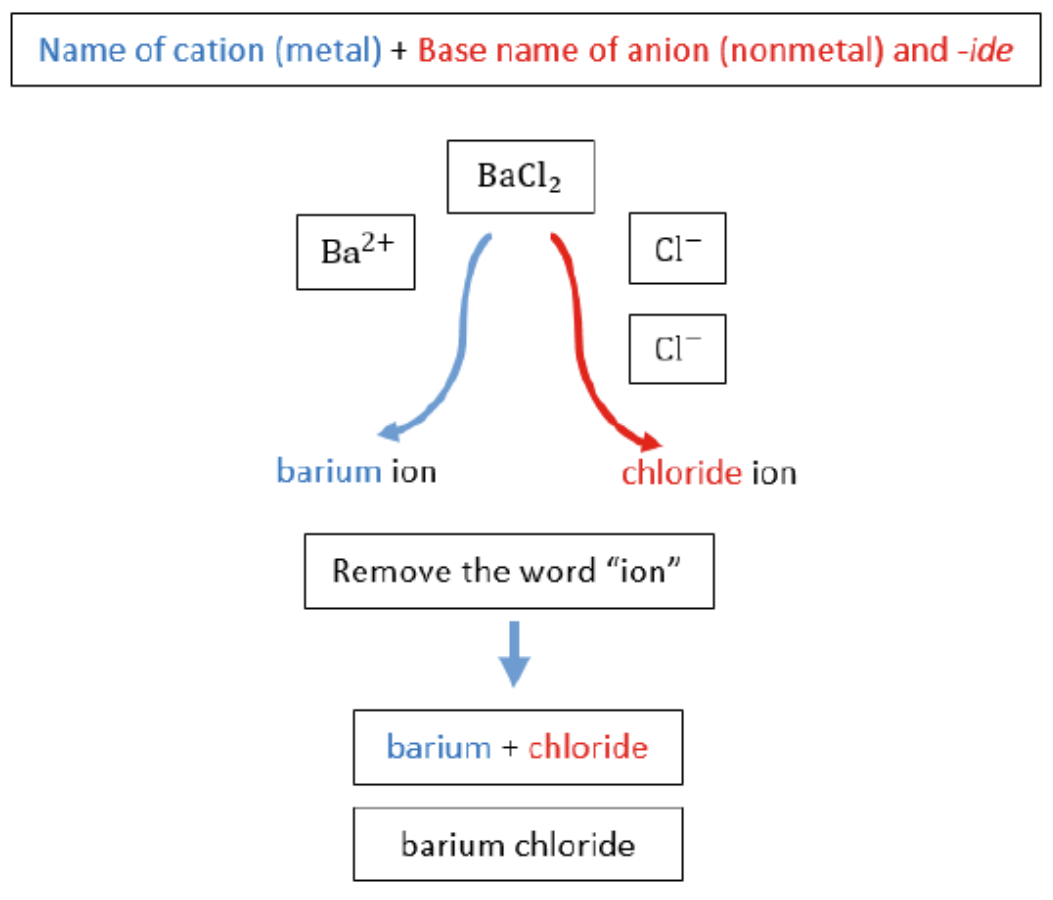
\includegraphics[width=0.7\linewidth]{barium_examp.png}
\end{frame}

\begin{frame}{Naming Molecular Compounds}
  \begin{center}
    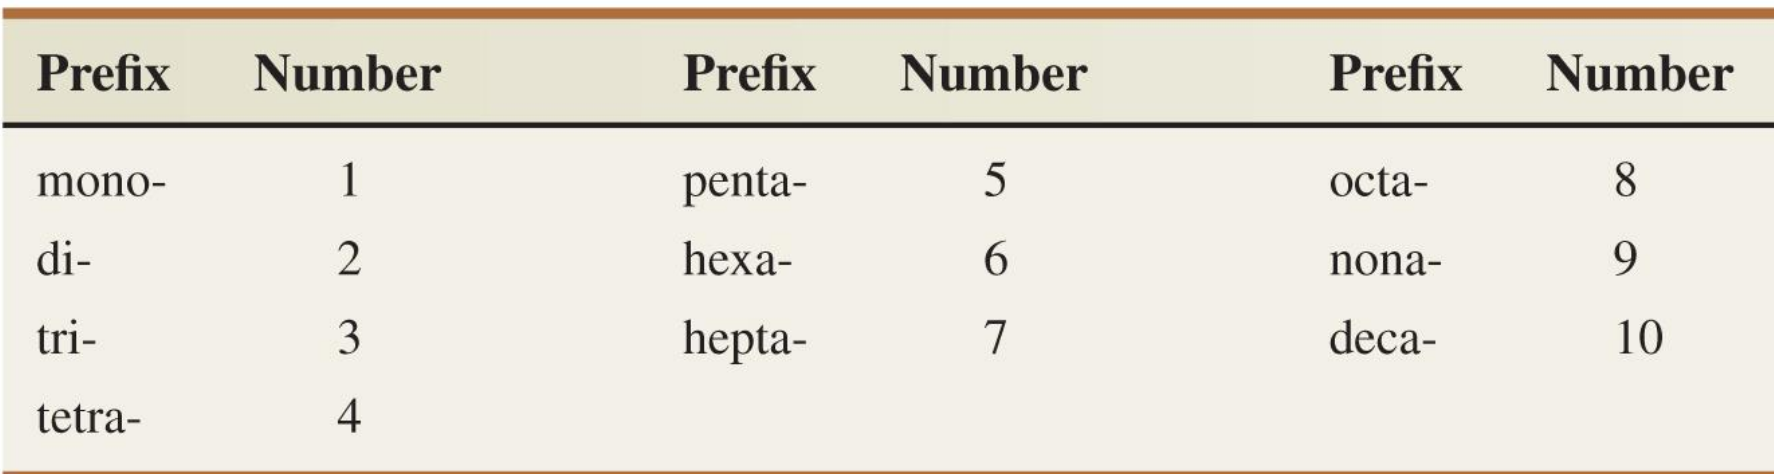
\includegraphics[width=\linewidth]{prefix_name}
  \end{center}
  
  \begin{enumerate}
  \item Use numerical prefix for the element (usually ignore the first
    when using ``mono'')
  \item Add ``-ide'' to the second element
  \end{enumerate}
\end{frame}

\begin{frame}{Naming Acids and Bases}
  \begin{center}
    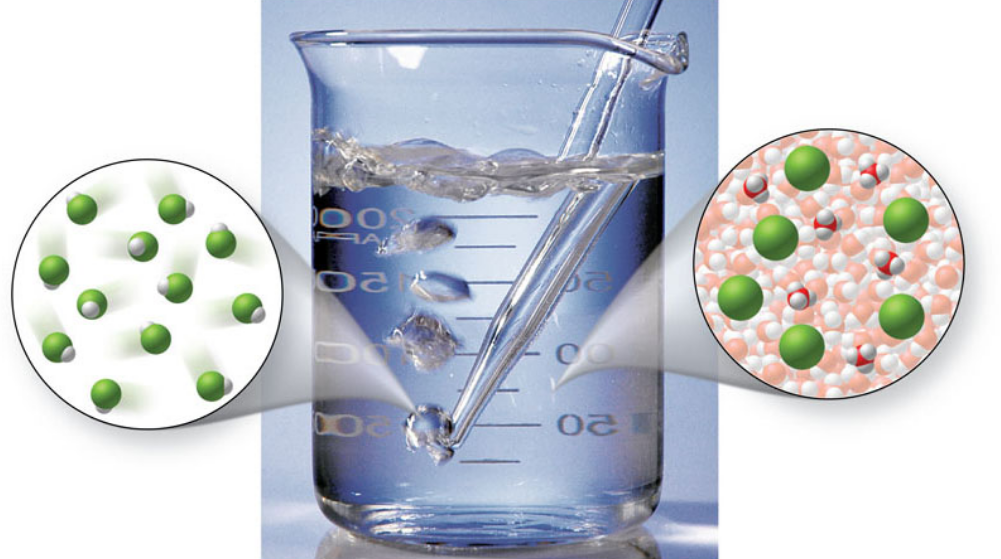
\includegraphics[width=0.5\linewidth]{acid_base}
  \end{center}

  \begin{enumerate}
  \item If anion ends in ``-ide,'' add ``hydro'' before the
    root of the anion name followed by ``-ic acid''
  \item If anion ends in ``-ate,'' use the root of the anion
    name followed by ``-ic acid''
  \item If anion ends in ``-ite,'' use the root of the anion
    name followed by ``-ous acid''
  \end{enumerate}
\end{frame}

\begin{frame}{Definition(s) of an Acid}
  \vspace{0.2in}
  \textbf{Arrhenius Acid} - dissociation of acid in water to yield
  the ions e.g. HCl(aq) $\rightarrow$ H$^+$(aq) + Cl$^-$(aq)
  
  \textbf{Br{\o}nsted Acid} - any species that can donate a proton
  H$^+$

  \begin{center}
    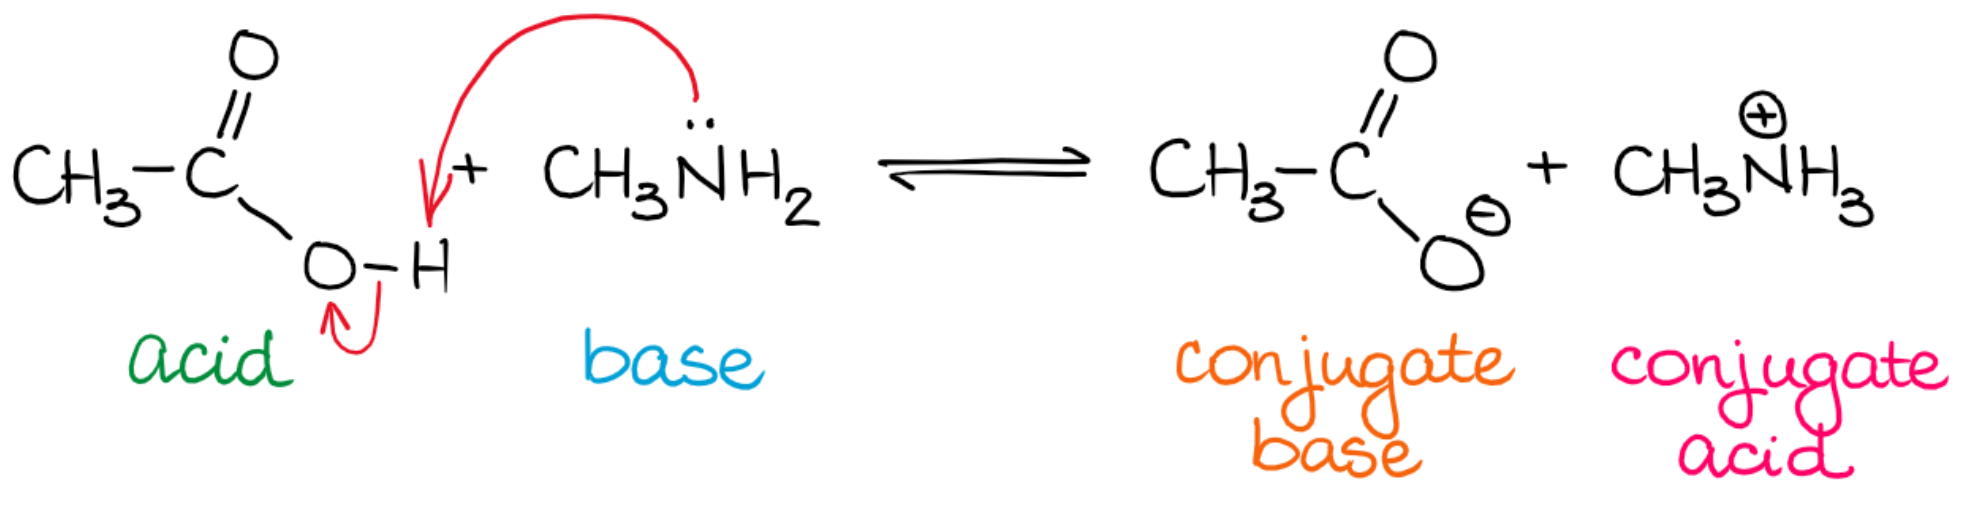
\includegraphics[scale=0.1]{bronsted_acid}
  \end{center}
  \vspace{-0.2in}
  \textbf{Lewis Acid} - donation of a pair of electrons
  \begin{center}
    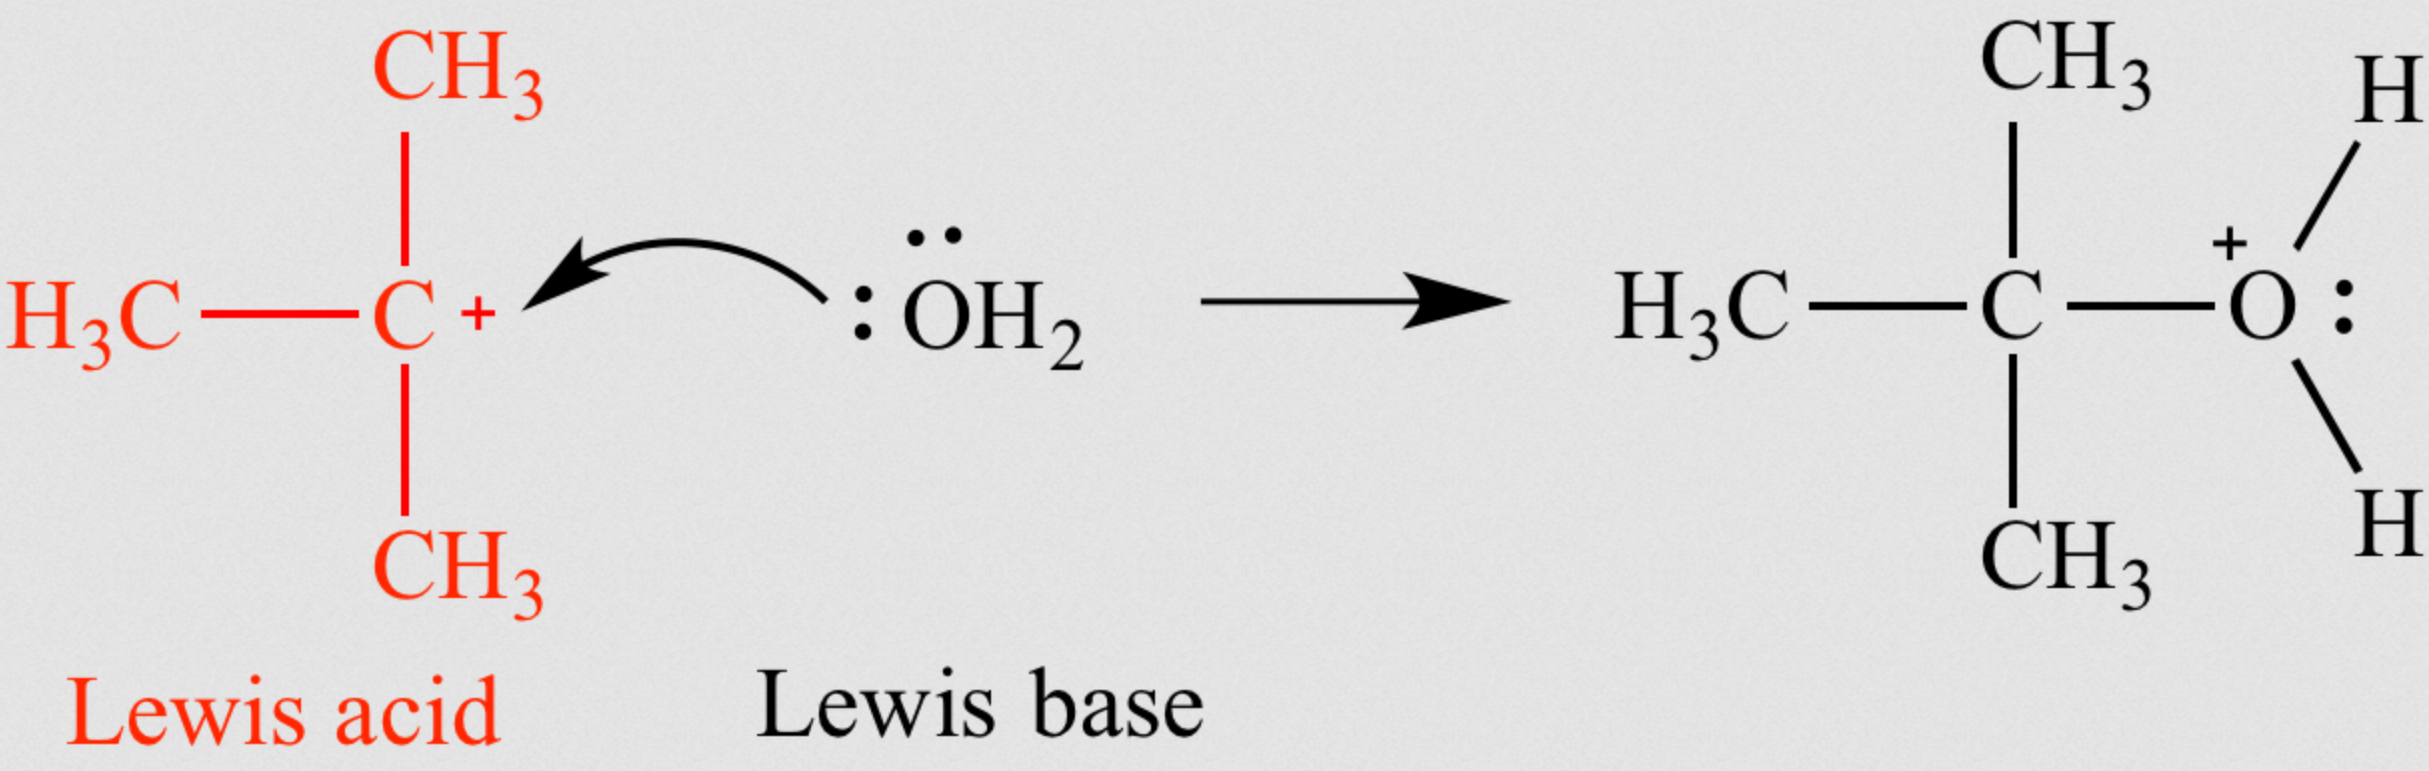
\includegraphics[scale=0.07]{lewis_acid}
  \end{center}
\end{frame}

\section{Percent Composition}

\begin{frame}{Percent Compsition}
  \textbf{Main Takeaway:} Convert the mass of each component
  to a percentage of the total mass

  \begin{equation}
    P_A = \frac{M_A}{M_\text{Tot}} \times 100\%
  \end{equation}

  where $M_\text{Tot}$ is the total mass, $M_A$ is the mass and $P_A$
  is the percent composition for component $A$
\end{frame}

\begin{frame}{Example Problem: Percent Composition}
  Magnetite, Fe$_3$O$_4$, is a mineral containing $72.4\%$ iron. What
  mass of iron is present in an 837g sample of magnetite?

  \begin{align*}
   \onslide<2->{ (837 \text{g magnetite})\frac{72.4 \text{g iron}}{100 \text{g magnetite}}
    = 606 \text{g iron}}
  \end{align*}
  
\end{frame}

\section{The Mole Concept}

\subsection{Determining Empirical and Molecular Formulas}

\begin{frame}{The Mole Concept}
  \begin{center}
    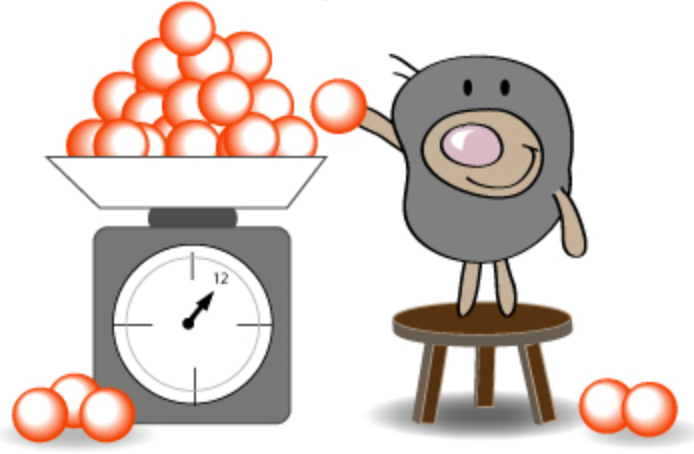
\includegraphics[scale=0.2]{mole}
  \end{center}
  
  \textbf{Q:} What is a mole (mol)?

  \textbf{A:} A mole is measurement of a substance and relates to
  Avogadro's number ($6.022 \times 10^{23}$)

  \textbf{side note:} Mole day is Oct. 23, between 6:02 a.m. and 6:02 p.m
\end{frame}

\begin{frame}{Purpose of the Mole}
  \begin{center}
    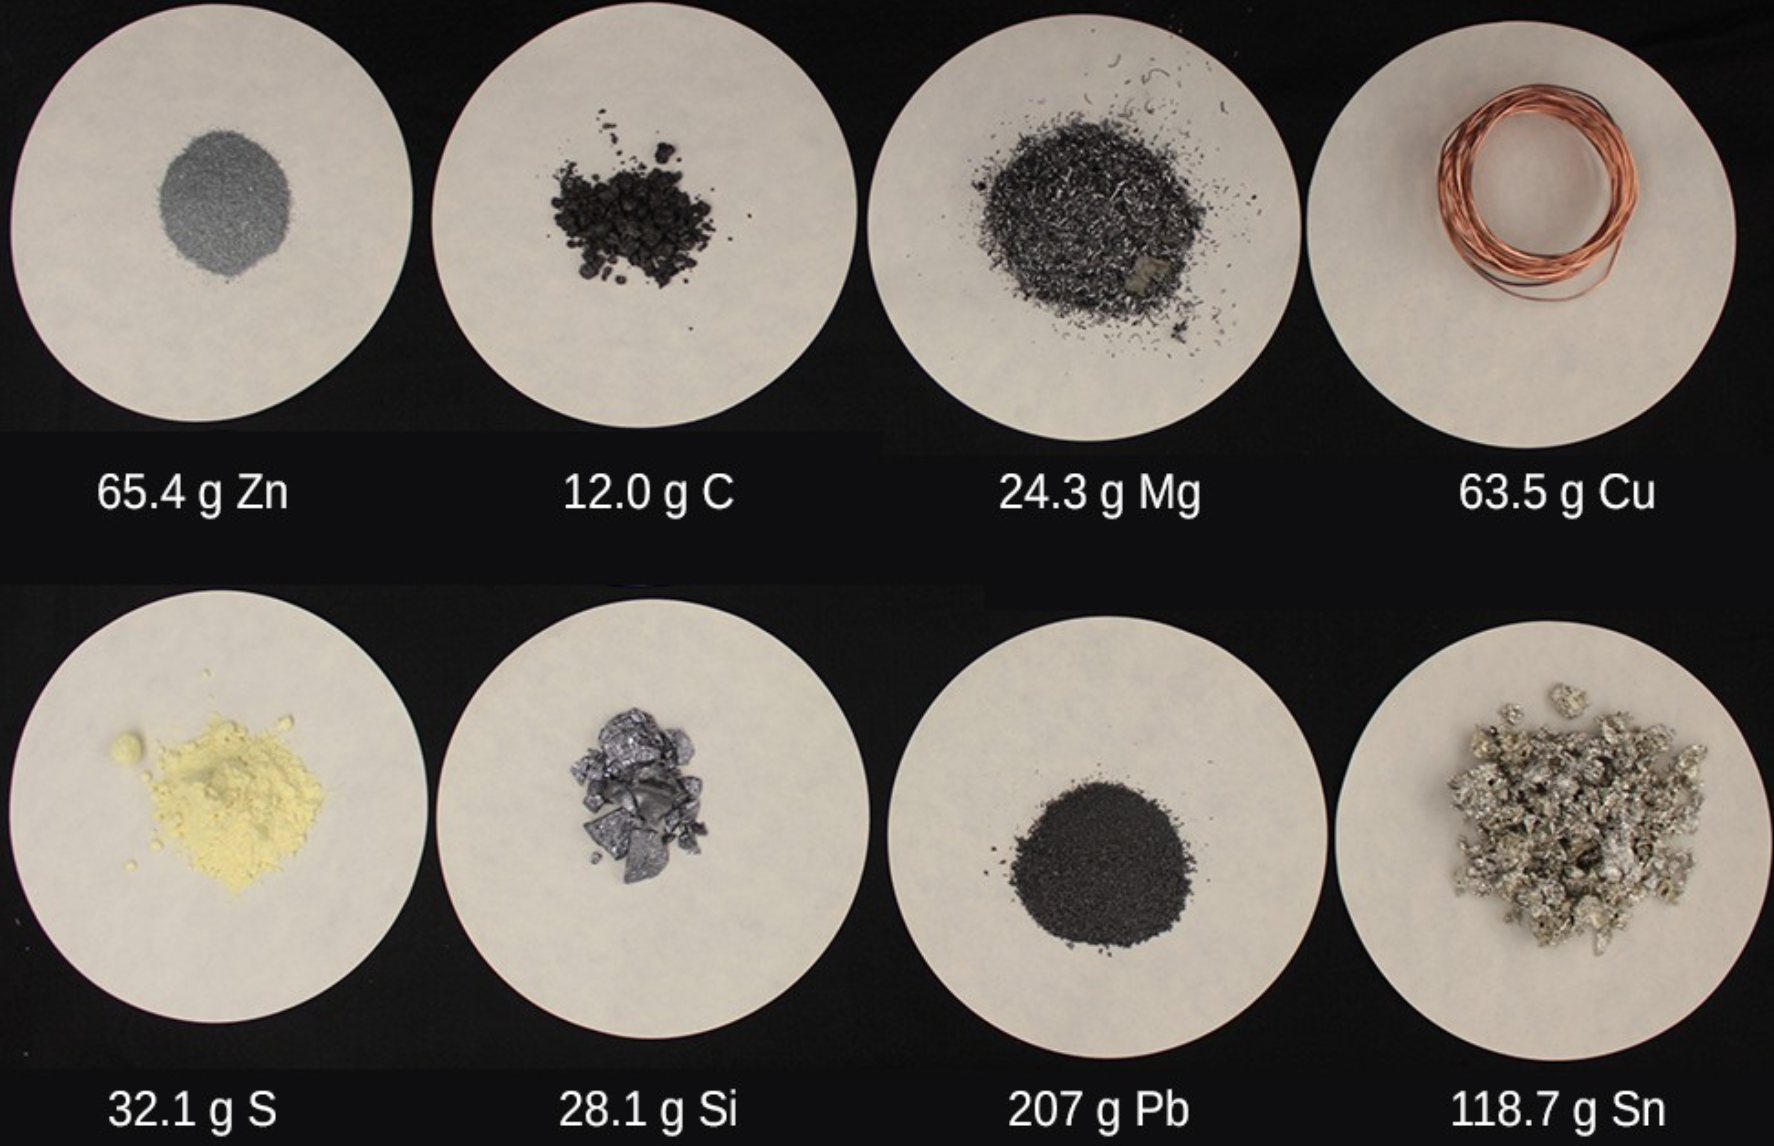
\includegraphics[scale=0.1]{mol_solids}
  \end{center}
  
  \begin{itemize}
  \item Gives a consistent method to convert between atoms/molecules and grams
  \item Convenient way to preform calculations
  \item View the mole (mol) as a unit conversion type approach
  \end{itemize}
\end{frame}

\begin{frame}{Reminder: Periodic Table}
  \centering
  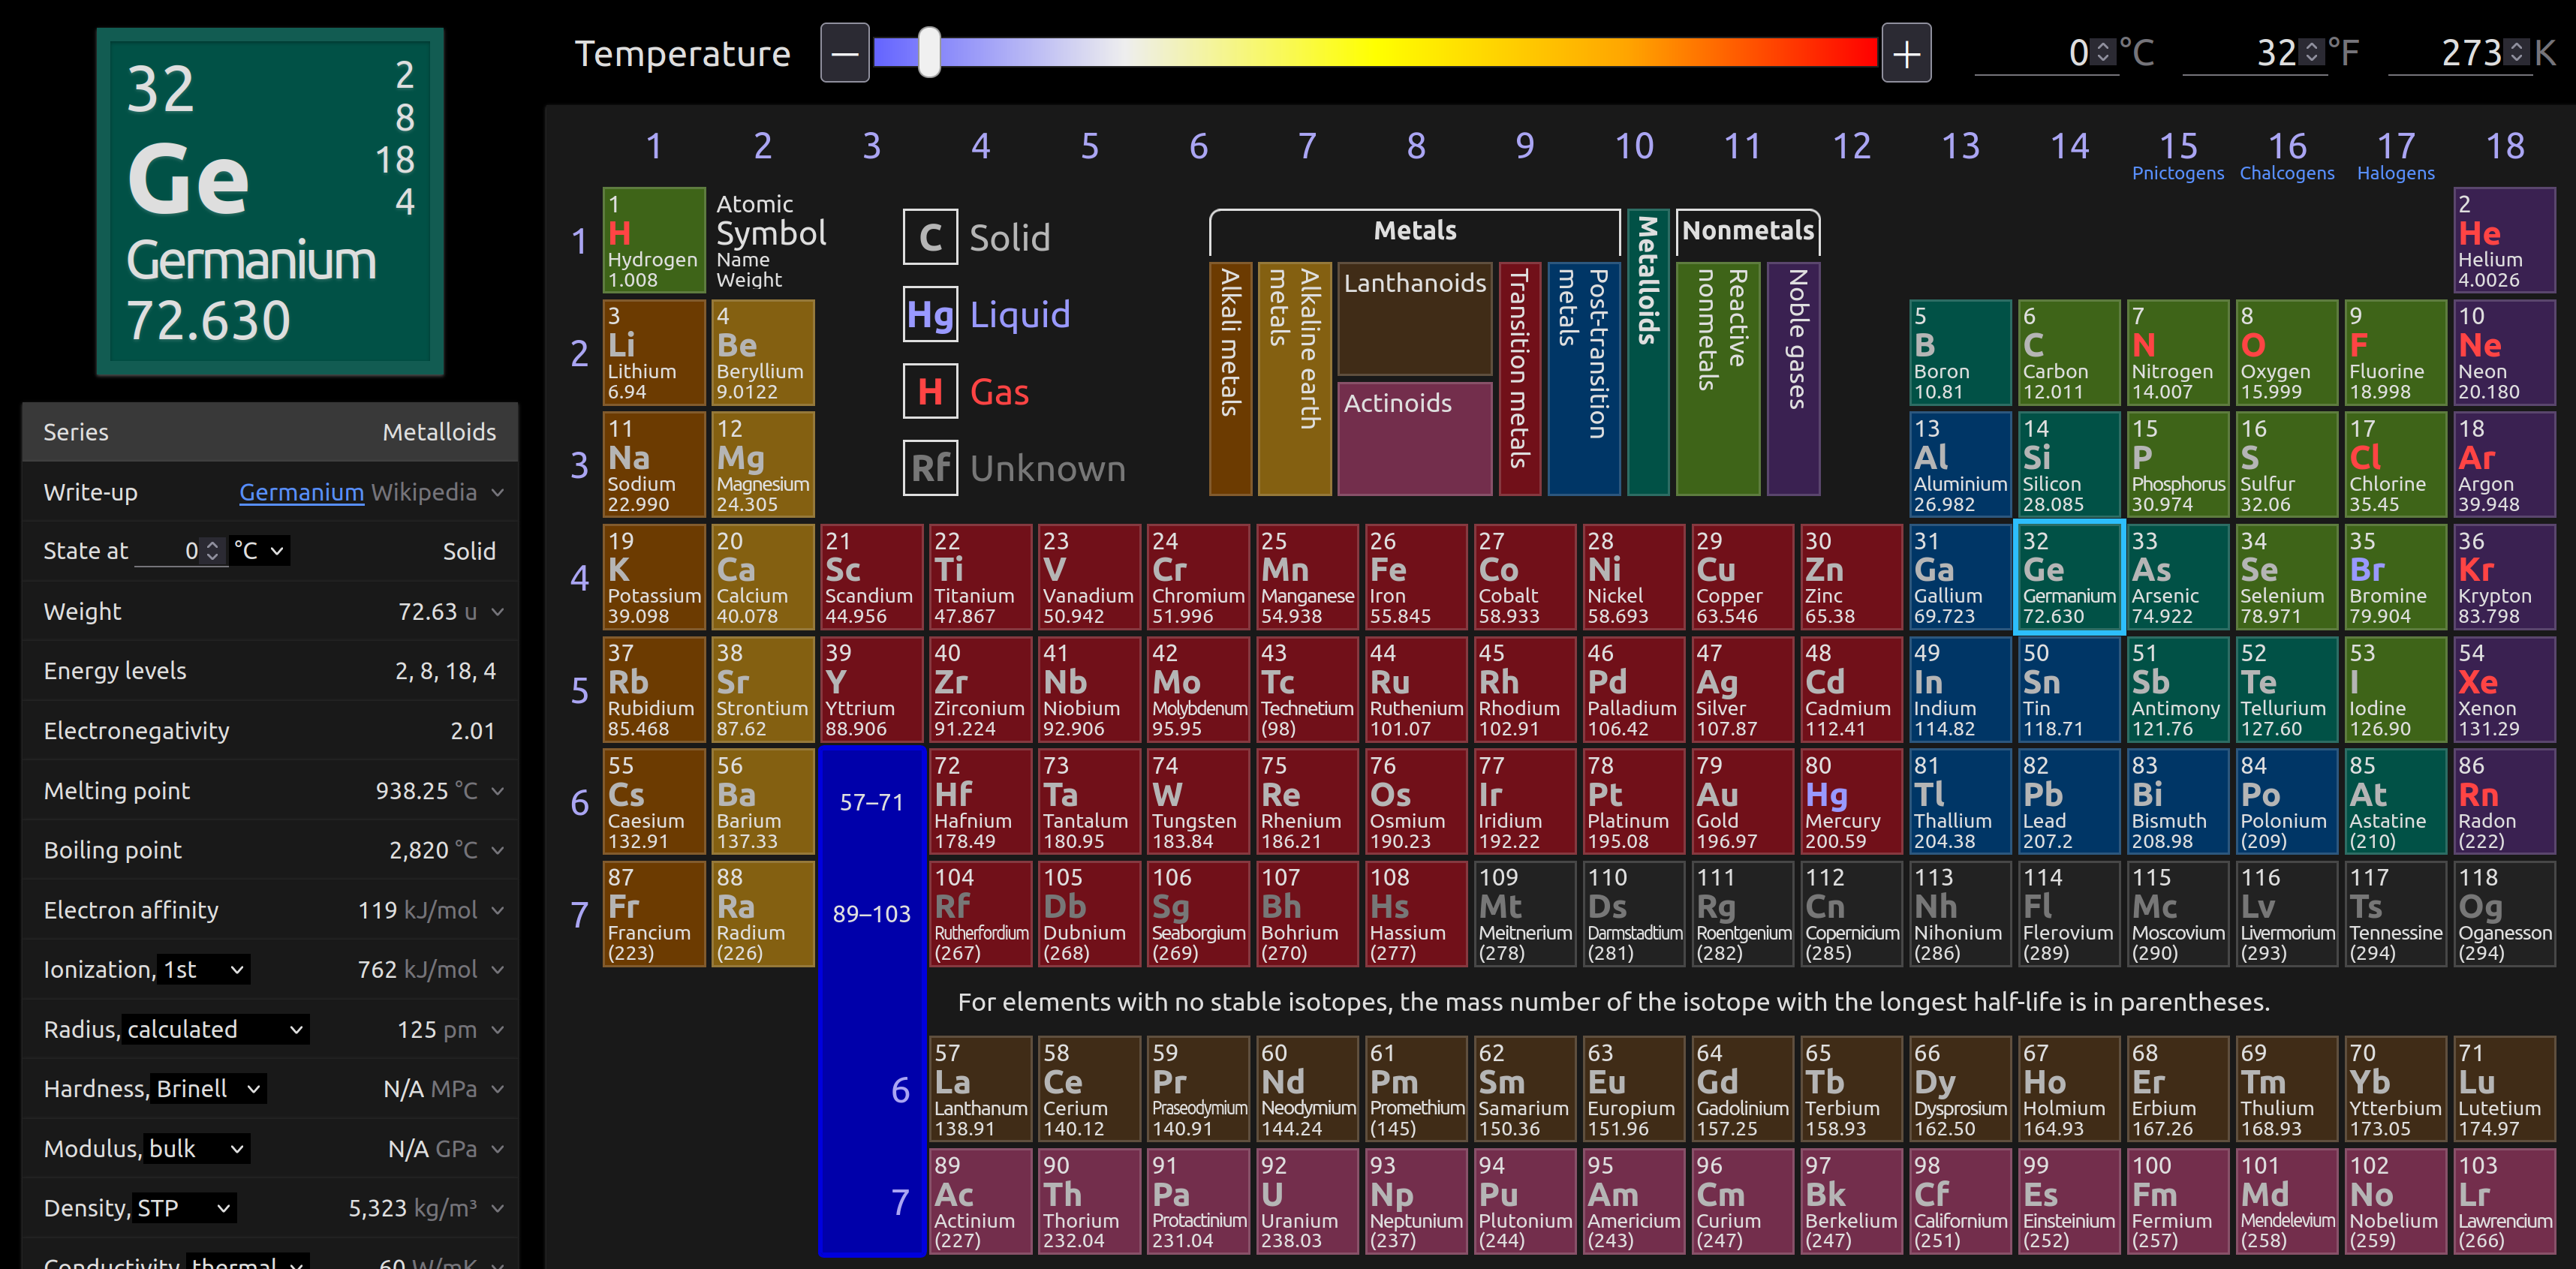
\includegraphics[width=\linewidth]{ptable}
\end{frame}

\begin{frame}{Example: Determine the mol of each element within a compound.}
  H$_2$O \onslide<2->{- 2 mols H and 1 mol O}
  
  C$_6$H$_{12}$O$_6$ \onslide<3->{- 6 mols C, 12 mols H, 6 mols O}

  \onslide<3->{\textbf{Concept:} Determine the molar masses}
\end{frame}

\begin{frame}{Example: Mole Connection to Chemical Rxn}
  Zn(s) + 2 HCl(aq) $\rightarrow$ ZnCl$_2$(aq) + H$_2$(g)

  \textbf{Q:} What are the mols of each reagent required to run this reaction?
  And how much mol of each product is produced?

  \onslide<2-> 2 mol Zn(s) and 2 mol HCl(aq) (reagents) produce 1 mol ZnCl$_2$(aq)
  and 1 mol H$_2$(g)
\end{frame}

\begin{frame}{Example: Combine Percent Composition and the Mole}
  Determine the mass percent of each element in Al$_2$(SO$_4$)$_3$.
  \small
  \begin{align*}
    \% \text{ mass of Al} & =
    \onslide<2->{\frac{n\times \text{molar mass Al}}{n \times \text{molar mass of Al$_2$(SO$_4$)$_3$}}
    \times 100\%\\
    & = \frac{2\times 26.98 \text{g}}{342.14 \text{g}} \\
    & = 15.77 \%} \\
    \onslide<3->{\% \text{ mass of S} & =
      \frac{n\times \text{molar mass S}}{n \times \text{molar mass of Al$_2$(SO$_4$)$_3$}}
    \times 100\%\\
    & = \frac{3\times 32.06 \text{g}}{342.14 \text{g}} \\
    & = 28.11 \% \\
    \% \text{ mass of O} & = \frac{n\times \text{molar mass O}}{n \times \text{molar mass of Al$_2$(SO$_4$)$_3$}}
    \times 100\%\\
    & = \frac{12\times 16.00 \text{g}}{342.14 \text{g}} \\
    & = 56.12 \% \\}
  \end{align*} 
\end{frame}

\begin{frame}{Practice: Determine Mass from Moles}
  A friend heats water in a copper kettle and makes a cup of tea. The
  friend adds 0.0120 mol of table sugar (sucrose, C$_{12}$H$_{22}$O$_{11}$).
  What mass of sugar has he added?
\end{frame}

\begin{frame}{Practice: Number of Molecules from Mass}
  A substance named Agorca M5640 is used for concentrating extracted
  copper ore. Its molecular formula is C$_{16}$H$_{25}$NO$_2$. If you have a
  150.0 g sample of Agorca M5640, how many molecules do you have?
\end{frame}

\begin{frame}{Defn: Empirical and Molecular Formulas}
  \textbf{Empirical Formula} - the simplest ratios of atoms in
  a compound; lowest possible ratio

  \textbf{Molecular Formula} - a factor of the empirical formula
\end{frame}

\begin{frame}{Approach for Empirical/Molecular Problems}
  \begin{itemize}
  \item Convert all elemental masses to mols
  \item Determine the lowest possible ratio
  \item Round to the nearest integer for each element and that
    number is the empirical formula
  \item For molecular formula, use the given experimental molar
    mass and divide by the molar mass of empirical formula. Multiply
    the empirical formula by that ratio.
  \end{itemize}
\end{frame}

\begin{frame}{Practice: Empirical Formula from Percent Composition}
  Determine the empirical formula for the mineral chalcocite, which has
  the percent composition $79.8\%$ Cu and $20.2\%$ S.
\end{frame}

%\section{Molarity of Solution}
%
%\subsection{Concentrations and Dilutions}

\end{document}
